\chapter{Hoome төсөл}

\hspace{0.5cm}
Үйлдвэрлэлийн дадлагын хүрээнд одоо идэвхитэй явагдаж буй "Hoome" төсөл дээр ажилласан бөгөөд энэхүү төсөл нь Hoome мобайл аппликейшн, Hoome сөх веб, Hoome контор веб зэрэг системүүдээс бүрдэх цогц систем юм. Одоогоор бүртгэлтэй 24000 хэрэглэгч байгаа ба тэдгээрийн 13000 нь идэвхитэй хэрэглэгч. 

Бизнесийн үйл ажиллагаа нь голчлон хэрэглэгчдийн өдөр тутмын амьдрал дээр тулгуурласан бөгөөд СӨХ-өөс гадна машины зогсоолын хэсгийг нэвтрүүлээд байгаа билээ. Зогсоолын хэсэг нь бие даасан систем бөгөөд CCP(Cloud Car Parking) гэх төслийн хүрээнд идэвхитэй хэрэгжиж байгаа болно. Уг системийг "Hoome" мобайл аппликейшнд feature байдлаар оруулж өгсөн байгаа. 

"Novelsoft" ХХК-ийн бүтээгдэхүүн болох "Homebook" СӨХ-ийн системийг сайжруулж сошиал коммунити аппликейшн болгож 2022 онд улмаар "Hoome" гэх шинэ төслийг эхлүүлсэн. 


% Бүлгийн дэд гарчиг
\section{Хотхон}
"Hoome" платформын хотхоны систем нь СӨХ-ийн менежмент, төлбөр, оршин суугчдын бүх төрлийн харилцааг удирдах тусгай систем болон түүнийг иргэдэд хүргэх "Hoome" сошиал аппын цогц бөгөөд
\begin{itemize}
  \item СӨХ-ийн төлбөр бодолт
  \item Хэрэглэгчийн төлбөр төлөлт
  \item Автомат иБаримт гаргах, илгээх
  \item Тайлан гаргах
  \item Хотхоны бүлгэм үүсгэх, сошиал пост, чат
  \item Оршин суугчдын жагсаалт, мэдээлэл, автомат бүртгэл
  \item Зогсоол, агуулах удирдлага
\end{itemize}
зэрэг функцуудээс бүрдэнэ.

\section{Контор}
"Hoome" платформын хотхоны систем нь конторын төлбөр бодолт, үйлчилгээний захиалга авах гэх мэт бүх үйл ажиллагааг удирдах, системтэй.
\begin{itemize}
  \item Бүх хэрэглэгчийн жагсаалт
  \item Конторын төлбөр бодолт
  \item Хэрэглэгчийн төлбөр төлөлт
  \item Тайлан гаргах
  \item Тоолуурын заалт
  \item Тариф удирдлага тохиргоо
  \item Автомат иБаримт гаргах, илгээх
\end{itemize}
зэрэг функцуудээс бүрдэнэ.

\section{Мобайл аппликейшн}
"Hoome" платформын мобайл аппликейшн нь СӨХ-ийн төлбөр төлөгч болон Hoome-д бүртгэлтэй зогсоолд машинаа тавьсан хэрэглэгчдэд зориулагдсан. Хэрэглэгч өөрийн хотхоны СӨХ-д элссэнээр сар бүрийн төлөх зардлууд болон тооцоог нэг дороос харах боломжтой болно. Зогсоолын төлбөр буюу "Cloud Car Parking" систем нь Hoome-д бүртгэлтэй зогсоолууд дээр машин тавьсан хэрэглэчийг төлбөрийг орсон хугацаанаас нь бодож тооцдог бөгөөд давхар orgware буюу хаалгач хүнийг ажиллуулдаг билээ. Тухайн зогсоолын төлбөрийг зөвхөн "Hoome" биш, зарим тохиолдолд "Toki" аппликейшнийн хэрэглэгчид аппликейшнээрээ дамжуулан төлбөрөө төлдөг бөгөөд энэ нь Hoome-CCP-ийн зэрэгцээ орших ижил төстэй систем болно.

Энэхүү асуудлыг шийдэхээр шийдэл дэвшүүлж дадлагын хугацаанд "Hoome" платформын front-end болон back-end хөгжүүлэлтүүдийг хийж гүйцэтгэсэн билээ. 

\begin{figure*}[ht!]
  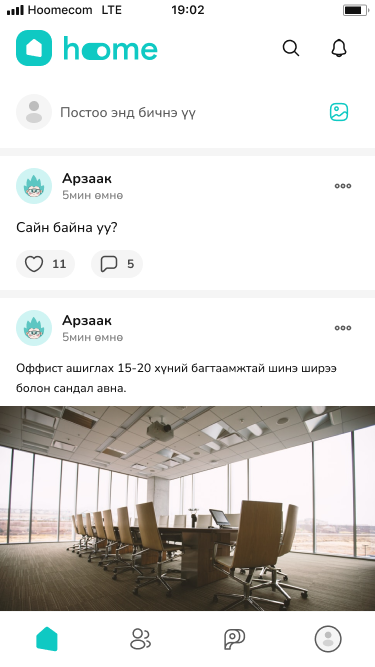
\includegraphics[width=.4\textwidth]{imgs/Home.png}\hfill
  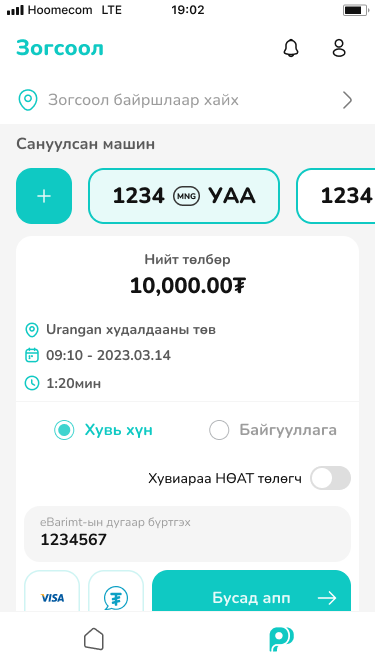
\includegraphics[width=.4\textwidth]{imgs/Parkly.png}
  \caption{Hoome - Коммунити нүүр.}
  \caption{Hoome - Cloud Car Parking нүүр.}
\end{figure*}